% BSPC V31 evidence-gated editorial candidate: keeps V24 verified history and adds the V31 NONSIGNIFICANT true acquisition result. NOT SUBMITTED.
% Original frozen cohorts and one newly executed but post-outcome Shin2017A comparator; see evidence hierarchy.
% Compile in paper_vnext, source files remain original and editable.
\documentclass[11pt,a4paper]{article}
\usepackage[margin=0.92in]{geometry}
\usepackage[T1]{fontenc}
\usepackage{amsmath,amssymb,booktabs,graphicx}
\usepackage{tikz}
\usepackage[hidelinks]{hyperref}
\usepackage{lmodern}
\usepackage[protrusion=true,expansion=false]{microtype}
\title{When Predictive Fit and Discriminative Transfer Disagree:\\
The Geometry of EEG Regularisation Selection}
\author{AUTHOR IDENTITIES AND AFFILIATIONS TO BE APPROVED}
\date{}
\begin{document}
\maketitle
\begin{abstract}
\textbf{Objective:}
Covariance fitting, Gaussian predictive likelihood, and
unknown-person EEG discrimination are different
regularisation objectives. We examine how a validation
estimand mismatch affects cross-subject conclusions,
and whether correcting or more precisely optimising
the source criterion improves transfer.

\textbf{Methods:}
A source-fitted tangent-space LDA pipeline is evaluated
under participant-grouped, zero-target-information
selection. We audit a historically labelled
covariance-NLL criterion, distinguish its
validation-class-centred score from true
source-mean predictive likelihood, and decompose
their exact difference into common-location,
score-orthogonal, and discriminant-aligned
class-mean shifts. Frozen positive, negative and
post-outcome source-only evidence is kept separate.

\textbf{Results:}
A prospectively frozen EEGMMIDB block (20 people)
showed a $+0.0561$ AUC gain for source-discrimination
selection over the historical class-centred score
(Holm $p=0.00597$), with five materially harmed
participants. In source-validation analyses of
Cho2017, Dreyer2023A and native-montage
BNCI2014\_002, respectively, 98.59\%,
99.29\% and 99.77\% of the corrected
predictive-score mean-shift gap was attributable
to components invariant to the tested fixed
classifier's within-person AUC. These
three mechanism analyses were \emph{post-outcome}.
A ten-person protocol-first Weibo2014 test found
identical held-person AUC for continuous and
27-point source selection (0.73141).
A 40-person Cho2017 sequential follow-up
gave an essentially zero overall source-envelope
gain ($-0.000053$ AUC), not a superior decoder.

\textbf{Conclusion:}
A mathematically proper Gaussian likelihood
can still primarily measure variation irrelevant
to an EEG discriminant's within-person ranking.
Correct estimands, source-selection information
boundaries and individual harms are central;
the tested more elaborate source-only selectors
have not shown stable transfer superiority.
\end{abstract}

\noindent\textbf{Keywords:} EEG; covariance shrinkage; cross-subject decoding;
motor imagery; model-selection validity; representation sensitivity.

\section{Introduction}
Cross-subject EEG decoding asks a model fitted on source participants to
generalise to a different individual, often without labelled calibration.
Tangent-space covariance features are established in EEG decoding
\cite{barachant2012riemannian}, and can be high dimensional even
when each participant contributes few examples. A stable covariance estimator is therefore
attractive, but the statistical criterion used to estimate a covariance
matrix is not the criterion used to judge held-person classification.
Ledoit--Wolf shrinkage is an established covariance estimator
\cite{ledoit2004}; regularised discriminant analysis selected against
predictive discrimination is also classical \cite{friedman1989}.
Consequently, selecting a shrinkage parameter by source discrimination
is not, in itself, our claimed methodological invention.

A more basic measurement question is what is actually being scored:
centring held source participants with their own class means produces a
covariance log score that does not equal the predictive Gaussian log score
under source-trained means. Confusing these objectives can create an
apparent advantage for discrimination-based selection. A corrected
comparator must be run on real EEG to determine whether the original
objective comparison survives. A separate prospective intervention asks
whether the selection criterion can alter a spectral representation
conclusion under the same target-information budget. Contemporary work proposes
new regularisation mechanisms and multi-paradigm transfer methods
\cite{miao2025freezing,morvay2026wbt,he2026cyclic}, while recent research highlights
how participant-level rather than trial-level evaluation can change the
interpretation of EEG model performance \cite{gil2026subjectvalidation}.
Qin and colleagues, in a recent study published in this journal,
evaluated spatial normalization with SVM decoding across nine
distinct EEG paradigms under within- and between-subject validation
\cite{qin2026spatialnorm}. That study provides stronger
cross-paradigm breadth than the fixed tangent-LDA family examined here.
Our narrower, complementary question is how the \emph{source
validation likelihood itself} changes the selected
regularisation regime; this is a measurement problem rather
than evidence of a superior novel classifier.
These contributions motivate our strict comparison but do not substitute
for an objective-controlled study.

We study a fixed tangent-space linear discriminant family, separating
three source-only selection targets: held-source-participant
macro-AUC, a validation-class-centred covariance score, and a true
Gaussian predictive score using only source-training class means.
The third comparator was executed on Shin2017A only after its original
target results had been seen; this is retrospective and is not part of
the frozen confirmatory family. All target labels, target feature
moments and target-fitted geometry are excluded from primary source-only
(Z0) selection. We preserve the original predeclared finite shrinkage grid,
frozen prospective test cohorts, the representation falsification,
individual harms, and the newly verified posterior comparator. An additional BNCI2014\_001 acquisition and a new Weibo2014
ten-person, three-channel dataset were evaluated under
repository-committed protocol-first procedures. Neither experiment
constitutes independent external preregistration.

The objective is not to show
that one numerical shrinkage value is universally optimal; it is to measure
how an incorrectly described covariance-validation estimand can change
the interpretation of a transfer comparison.


% Accepted BSPC 2025--26 head-to-head editorial audit.
% This is comparative research context, NOT a same-protocol accuracy leaderboard.
\subsection{What recent accepted EEG studies actually establish}
\label{sec:bspc-headtohead}
An assessment against previously published biomedical
signal-processing studies must distinguish a
\emph{new high-performing decoder} from a
\emph{new evaluation/measurement claim}.
The most informative analogues are not exclusively
large EEG networks. In BSPC, Gil and
Hern\'andez-Sabat\'e \cite{gil2026subjectvalidation}
tested six models under window-, state-, and
participant-level EEG seizure validation:
window-level mean recall/specificity of
$0.96/1.00$ fell to $0.77/0.90$ at the
participant level. Their hierarchical mixed-effects
analysis experimentally demonstrated that evaluation
unit changes the scientific conclusion.
Qin \emph{et al.}\ \cite{qin2026spatialnorm}
tested spatial normalization across nine EEG
ERP/cognitive paradigms. They reported an
average between-participant decoding effect
size of Cohen's $d=1.39$ ($p<0.001$), but
not a comparable within-participant improvement,
and independently inspected morphology of
the EEG difference waves.
Those studies demonstrate that rigorous
\emph{measurement/validation research} is a
legitimate BSPC contribution, but their
experimental reach and actionable consequences
also impose a high standard.
Our three-acquisition source-only
held-group analysis has exact decompositions
and independent artifact reproducibility,
but has not established an analogous broad
\emph{new-target} prospective benefit.

Recent cross-domain decoder studies address
different information budgets.
Zhang \emph{et al.}\
\cite{zhang2025crossdataset_gcn}
used 62-channel teacher features, eight-channel
student transfer, labelled target-session
fine-tuning, and channel-count/transfer ablations.
Its accepted-author manuscript compares CSP,
FBCSP and multiple neural models, and reports
eight-channel target classification accuracies
of $71.19\%$ in cross-validation and
$69.03\%$ in the cross-session scenario
\emph{after} target adaptation.
Morvay \emph{et al.}\
\cite{morvay2026wbt}
combined Wasserstein barycenter transport
with four classifiers across three
EEG datasets and four tasks; their
unsupervised adaptation uses the
\emph{unlabelled target recording} when
mapping source to the new subject.
The study reports 79.59\% balanced accuracy
on VEPESS \emph{visual evoked potential}
data and 53.97\% MI accuracy on
BCIC4D2a; the two tasks themselves
must not be conflated.
Our original EEG estimand tests instead
enforce zero held-target signal \emph{or}
labels during source model selection.
Therefore neither post-adaptation accuracy,
cross-task balanced accuracy nor our
person-macro binary ROC-AUC
is an equal-information performance ranking.

\begin{table}[tb]
\centering\small
\caption{Published BSPC EEG evidence versus the present
zero-target-information scientific question.
The entries describe \emph{study design}, not
a directly comparable leaderboard:
datasets, task and metrics can differ.}
\label{tab:bspc-paper-budget}
\setlength{\tabcolsep}{3.2pt}
\begin{tabular}{p{.24\linewidth}p{.34\linewidth}p{.30\linewidth}}
\toprule
Published work & Verification/breadth & Target information\\
\midrule
Gil et al., 2026 \cite{gil2026subjectvalidation}
& Six networks, seizure EEG, three split levels
& Participant held-out evaluation\\
Qin et al., 2026 \cite{qin2026spatialnorm}
& Nine ERP paradigms, subject-level effects,
waveform morphology
& Within/between-person analyses\\
Zhang et al., 2025 \cite{zhang2025crossdataset_gcn}
& 62-to-8-channel transfer, CSP/FBCSP,
deep baselines and ablations
& Target-labelled fine-tuning\\
Morvay et al., 2026 \cite{morvay2026wbt}
& Three datasets, four tasks, four
classifiers; MI and VEP
& Unlabelled target-domain transport\\
Murtaza et al., 2025 \cite{murtaza2025signature}
& EEG channel-correlation intersubject
distance and source similarity
& Resting EEG may inform new-subject similarity\\
This study
& Exact three-factor score anatomy on
three exposed source acquisitions;
frozen positive and negative outer studies
& Zero target signal/labels for source selection\\
\bottomrule
\end{tabular}
\end{table}

The neural-signature distance study by
Murtaza \emph{et al.}\ \cite{murtaza2025signature}
is especially relevant: a measured
cross-participant quantity is valuable partly
because it can inform subject similarity
and downstream transfer. A large
AUC-invariant source-likelihood penalty
in our analysis is not yet an \emph{actionable}
source-to-unseen-target predictor.
Further BSPC studies offer complementary
standards: cyclic domain adaptation
\cite{he2026cyclic} tests new EEG
representations, while DLSSNet
\cite{wang2026dlssnet} combines
high-accuracy decoding with interpretable
sensorimotor-rhythm temporal states.
The reported DLSSNet BCI2a and
High Gamma accuracies of 78.51\%
and 95.49\%, respectively, cannot
be directly compared with a different
zero-target person-macro ROC-AUC.
For a stronger algorithm manuscript,
our method would need a genuinely distinct
selected operator, matched CSP/FBCSP and
Riemannian/linear controls, an explicit
target-information ledger, paired new-person
effect sizes, and prospective replication
under at least two independently recorded
acquisitions. Neither the classical
three-factor identity nor the
currently unsupported V31/V32 improvements
satisfies those requirements.

\paragraph{Novelty limit relative to accepted studies.}
The exact quadratic decomposition is
standard linear algebra, and the
prevalence of participant-location shifts
in our released data is a descriptive,
post-outcome source-validation observation.
Our supported potential contribution is
the EEG-specific \emph{estimand mismatch and
its independently audited implications
for interpreting source-only regularisation},
not a newly proven globally optimal
EEG decoder, a transfer guarantee or
stronger performance than established
BSPC networks.


\section{Methods}
\subsection{Datasets and target-information budgets}
PhysioNet EEGMMIDB S001--S008 is the method-development source pool
\cite{schalk2009eegmmidb,schalk2004bci2000}.
Its S021--S040 participants form a prospectively untouched target block
of 20 people. The primary fixed 21-channel sensorimotor montage, 8--30 Hz
filtering and source-fitted Riemannian tangent reference generate 231
wide-band coordinates. The independently frozen BNCI2014\_002
(\(N=14\), 15 channels, 120 features) and BNCI2015\_001
(\(N=12\), 13 channels, 91 features) protocols use native montage,
8--30 Hz processing and leave-one-person-out evaluation. Shin2017A
(\(N=29\), 30 channels, 465 features) was frozen under a \emph{separate}
prospective protocol before that cohort's target outcomes and is not a
retrospective addition to the original BNCI inference family.

All main effects use Z0: no target labels, target feature means, target
covariance, target normalisation statistics or target-selected feature
configuration. Within each source-validation fold, tangent references and
other representation-dependent operations are refitted using available
source participants only. Repeated trials and sessions do not become
independent inferential units.

\subsection{Paired objectives on one scalar shrinkage path}
For source within-class covariance \(S\), let
\[
 A_\lambda=(1-\lambda)S+\lambda\nu I,\qquad
 \nu=\mathrm{tr}(S)/p,\quad \lambda\in[0,1].
\]
Two source objectives are evaluated on the same participant-grouped folds:
macro-AUC \(A_s(\lambda)\), maximised for discrimination, and held-source validation-class-centred covariance log score
\(C_s(\lambda)\), minimised for within-class covariance fit.
This frozen estimator historically appears in logs and tables as
Cov-NLL, but it uses each held-source validation participant's own
class-centred residuals; it is not a source-mean predictive likelihood
(Section~\ref{sec:v16-estimand-audit}). Analytic Ledoit--Wolf and OAS shrinkage use the same
source feature pool; tangent-space logistic regression and Riemannian
MDM serve as additional non-identical algorithm controls. Full-domain
selection refers to the \emph{finite} 27-point candidate grid
\[
\begin{aligned}
\Lambda=\{&0,.0005,.001,.002,.003,.005,.0075,.01,.015,\\
&.02,.03,.05,.075,.10,.15,.20,.30,.40,.50,\\
&.60,.70,.80,.90,.95,.98,.99,1\}.
\end{aligned}
\]
Singular candidates are declared infeasible, not silently replaced by
a target-informed rule. Target scores are frozen before their
label-based performance is calculated.

\subsection{A critical estimand distinction: class-centred covariance score versus predictive NLL}
\label{sec:v16-estimand-audit}

An audit of the \emph{original executed} Shin2017A/BNCI2014\_002
source-selection code found a material distinction between the
frozen baseline's historical name and its actual measurement
quantity. The original program performs source-participant-grouped
validation, forms within-class residuals from \emph{the held source
validation participant's own labelled class means}, and evaluates
a covariance Gaussian log score on those residuals.
These source-participant labels are permitted for model development
and do \emph{not} imply outer target-subject label leakage.
However, the resulting number is not a proper predictive
class-conditional log likelihood under source-fitted class means.

To be precise, write the source-trained regularised within-class
covariance as $A_\lambda$, and for held source participant $g$
let $\widehat\mu_{g,c}$ be the \emph{held} participant's
empirical mean for class $c$. Up to additive constants, the
original finite-sample validation score is
\begin{equation}
\label{eq:v16-centred-score}
 C_{\mathrm{cent},g}(\lambda)=\frac{1}{p}
 \left[
  \log|A_\lambda|+
  \frac{1}{n_g}\sum_{i=1}^{n_g}
  (x_{gi}-\widehat\mu_{g,y_{gi}})^\top
  A_\lambda^{-1}(x_{gi}-\widehat\mu_{g,y_{gi}})
 \right].
\end{equation}
The source criterion in the frozen experiments is the
grouped average of $C_{\mathrm{cent},g}(\lambda)$,
and all existing performance tables retain its original
method identifier \texttt{source\_cov\_nll\_full\_domain\_LDA}.
For readability we call it the
\emph{class-centred covariance-score selector (CovScore)}
hereafter. Historical Cov-NLL column labels refer
to this exact frozen estimator, not to the new comparator below.

A \emph{genuinely held-source predictive} Gaussian
class-conditional score would instead evaluate
\begin{equation}
\label{eq:v16-conditional-prediction}
 C_{\mathrm{pred},g}(\lambda)=\frac{1}{p}
 \left[
  \log|A_\lambda|+
  \frac{1}{n_g}\sum_{i=1}^{n_g}
  (x_{gi}-\widehat\mu_{\mathrm{train},y_{gi}})^\top
  A_\lambda^{-1}(x_{gi}-\widehat\mu_{\mathrm{train},y_{gi}})
 \right],
\end{equation}
with the class means and covariance fitted from
\emph{the source training groups only}, without refitting
the held group's means. The source-validation labels
index the corresponding training-class mean; they are
not used to estimate it. Equation~\eqref{eq:v16-conditional-prediction}
is a different comparison protocol, \emph{not}
the estimand evaluated in the original frozen
EEGMMIDB/BNCI/Shin result tables. A later \emph{post-outcome}
real EEG execution of this corrected source-only criterion
on Shin2017A is reported separately in
Section~\ref{sec:v18-fair-predictive}; it is not
part of any original prospective testing family.

\paragraph{Proposition (class-contrast shift blind spot).}
Consider any fixed held-source validation data with
at least one observation in each class, and apply an
arbitrary class-specific feature translation
$x'_{gi}=x_{gi}+b_{y_{gi}}$.
Then \emph{for every feasible} $\lambda$,
\[
 C'_{\mathrm{cent},g}(\lambda)
 = C_{\mathrm{cent},g}(\lambda).
\]
In contrast, $C_{\mathrm{pred},g}$ is generally changed
because the source-trained class means stay fixed.
Consequently, $C_{\mathrm{cent}}$ by construction
cannot measure conditional mean-contrast drift through
its held-source covariance log score.

\emph{Proof.} After translation,
$\widehat\mu'_{g,c}=\widehat\mu_{g,c}+b_c$,
so each residual
$x'_{gi}-\widehat\mu'_{g,y_{gi}}=
x_{gi}-\widehat\mu_{g,y_{gi}}$
is identical to its original value. The log-determinant
term does not depend on the held means. For the
predictive score, the source-fitted
$\widehat\mu_{\mathrm{train},c}$ does not shift and
the residual gains $b_c$ in general, changing its
quadratic form.\hfill$\square$

An exact numerical regression now computes both quantities
on identical synthetic training/validation splits, then
imposes class-conditional shifts. The historical
class-centred score remains equal to floating-point
precision along the entire $\lambda$ path, while
proper predictive log score changes. This
\emph{does not} prove that one of the two selectors
will improve EEG transfer; such a claim would require
a fresh source-only, pre-specified, held-person
experiment with the new comparator.

\paragraph{Interpretational consequence.}
The prospective finding in the present paper remains
a comparison of \emph{source participant discrimination}
against \emph{class-centred covariance fit} and
against analytic Ledoit--Wolf. The measured gain
relative to the frozen Cov-NLL code remains
numerically unchanged, but should no longer be described
as showing superiority over every possible covariance
predictive likelihood criterion.
This distinction also restricts the operator mechanism:
the derivative of the covariance quadratic form
is a conditional calculation at a fixed covariance,
not evidence that Eq.~\eqref{eq:v16-centred-score}
evaluates out-of-sample class-conditional density
with source-only class means. Source-only diagnostics
from the two definitions must never share an
ambiguous NLL field without their
residual-centring provenance.

\subsection{The exact missing term in the historical covariance-score criterion}
\label{sec:v17-mean-shift-decomposition}
The distinction between a validation-class-centred Gaussian
covariance score and a genuine source-trained-mean predictive
log score can be made \emph{exact}, rather than relying only
on a synthetic translation counterexample.

For one held \emph{source} validation person $g$ with $n_g$
examples in $p$ dimensions, let
$\widehat\mu_{g,c}$ denote its empirical class means,
$\widehat\mu_{\mathrm{train},c}$ the means fitted exclusively
on the source-training people, and
$\Delta_{g,c}=\widehat\mu_{g,c}-
\widehat\mu_{\mathrm{train},c}$. For any common,
source-fitted positive definite regularised covariance
$A_\lambda$, the two V16 criteria satisfy
\begin{equation}
\boxed{
 C_{\mathrm{pred},g}(\lambda)
 =
 C_{\mathrm{cent},g}(\lambda)
 +\frac{1}{p}\sum_{c\in\{0,1\}}
 \frac{n_{g,c}}{n_g}
 \Delta_{g,c}^\top A_\lambda^{-1}\Delta_{g,c}.
}
\label{eq:v17-exact-nll-shift}
\end{equation}
The additional term is \emph{nonnegative} and
becomes zero exactly when the validation class means
match the training class means, for all classes present.
It is a covariance-weighted \emph{source-person
class-mean shift penalty}, not a regularisation
term chosen by target data.

\emph{Proof.} For each validation trial of class $c$,
decompose
$x_{gi}-\widehat\mu_{\mathrm{train},c}=
(x_{gi}-\widehat\mu_{g,c})+\Delta_{g,c}$.
Expand the quadratic form under $A_\lambda^{-1}$.
The cross term vanishes within each class because
$\sum_{i:y_i=c}(x_{gi}-\widehat\mu_{g,c})=0$.
Both log-determinant terms agree, and the remaining
class-mean quadratic terms give
Eq.~\eqref{eq:v17-exact-nll-shift}.\hfill$\square$

The penalty is $\lambda$-dependent because it measures
class-mean drift in the metric induced by $A_\lambda^{-1}$.
Its derivative can have \emph{either} sign:
\[
 \frac{\partial}{\partial\lambda}
 \bigl(C_{\mathrm{pred},g}-C_{\mathrm{cent},g}\bigr)
 =-\frac1p\sum_c\frac{n_{g,c}}{n_g}
 \Delta_{g,c}^\top A_\lambda^{-1}
 (\nu I-S)A_\lambda^{-1}\Delta_{g,c}.
\]
It follows that the proper predictive criterion
can select more \emph{or} less shrinkage than
the class-centred comparator. Merely asserting
that predictive selection is stronger or always
more regularised is unsupported. An independent
executable test verifies the identity for 300
randomly generated full-rank covariance operators,
multiple feature dimensions and source/validation
class-mean shifts, without using any held outer
target EEG data.

The identity provides a mechanistic interpretation
of the V16 estimand audit: the old frozen covariance
selection scores how well $A_\lambda$ describes
\emph{within-class residual fluctuations} in a
held source person; the correctly predictive version
also penalises \emph{between-source-person class-mean
misalignment}. This is not a newly invented
covariance estimator, and it does not establish that
minimising the added penalty improves held-person AUC.
A real, correctly nested evaluation of this second
source-selection criterion remains essential.

% New exact two-component decomposition of the ALREADY-AUDITED
% historical class-centred vs proper predictive source validation NLL.
% The identity is a classical weighted variance decomposition.
% No new target AUC gain or original-theorem priority is claimed.
\subsection{Disentangling transfer-relevant contrast from AUC-invariant location}
\label{sec:bspc-twofactor}
The exact predictive-minus-class-centred score term in
Eq.~\eqref{eq:v17-exact-nll-shift} still mixes two statistically
distinct source-person shifts. This matters because a
Gaussian predictive density, even when correctly evaluated,
is \emph{not} a proper score for within-person ROC-AUC:
a common source-to-validation-person location shift may
lower predictive likelihood without changing any within-person
classification ranking.

Let $\pi_{g,c}=n_{g,c}/n_g$,
$\delta_{g,c}=\widehat\mu_{g,c}-
\widehat\mu_{\mathrm{train},c}$,
$\bar\delta_g=\pi_{g,0}\delta_{g,0}+
               \pi_{g,1}\delta_{g,1}$,
and $\Gamma_g=\delta_{g,1}-\delta_{g,0}$.
For the \emph{same} source-fitted positive definite
$A_\lambda$, the weighted parallel-axis identity gives
\begin{align}
C_{\mathrm{pred},g}(\lambda)
-C_{\mathrm{cent},g}(\lambda)
&=P_{\mathrm{loc},g}(\lambda)
  +P_{\mathrm{contrast},g}(\lambda),\label{eq:twofactor}\\
P_{\mathrm{loc},g}(\lambda)
&={\bar\delta_g^\top A_\lambda^{-1}\bar\delta_g\over p},\\
P_{\mathrm{contrast},g}(\lambda)
&={\pi_{g,0}\pi_{g,1}\over p}
  \Gamma_g^\top A_\lambda^{-1}\Gamma_g.
\end{align}
Both terms are nonnegative. The identity is exact for
\emph{finite} class-imbalanced samples and every
feasible $\lambda$; it requires no Gaussian data
assumption to hold as a squared-residual statement.

\paragraph{Proof and the AUC-invariant counterfactual.}
Substitute
$\delta_{g,0}=\bar\delta_g-\pi_{g,1}\Gamma_g$ and
$\delta_{g,1}=\bar\delta_g+\pi_{g,0}\Gamma_g$ into
Eq.~\eqref{eq:v17-exact-nll-shift}. The weighted cross
terms cancel exactly. If the held person's feature
vectors are all shifted by the same $b\in\mathbb R^p$,
then $\bar\delta_g$ becomes $\bar\delta_g+b$ but
$\Gamma_g$ is unchanged. For any fixed linear
score $f_w(x)=w^\top x+c$,
\[
 f_w(x^+ +b)-f_w(x^- +b)
 = f_w(x^+)-f_w(x^-),
\]
so the held-person ROC-AUC and all paired ranking
decisions remain identical \emph{regardless} of the
change in $P_{\mathrm{loc},g}$. The historical
held-class-centred score is invariant as well.
Thus $P_{\mathrm{loc},g}$ can grow without bound
under source-group location shifts that have no
effect on within-person AUC. A proper predictive
Gaussian NLL, though correct as a density score,
can therefore be a poor surrogate for
discriminative transfer under zero-target
information conditions.\hfill$\square$

\paragraph{Why retaining only the contrast term is insufficient.}
Even $P_{\mathrm{contrast},g}$ is only a class-mean
density discrepancy, not a guaranteed change in ROC-AUC.
For a fixed classifier $w$, an arbitrary class-contrast
displacement orthogonal to $w$ can increase
$P_{\mathrm{contrast},g}$ while keeping all
held-person scores and ranks identical.
For example, at $\lambda=1$, let the trained
mean contrast be $(2,0)$ in two-dimensional
feature space. The classifier is parallel to
the first coordinate. Moving the validation
positive-class mean by $(0,h)$ for any $h$ leaves
all classifier scores unchanged but increases
$P_{\mathrm{contrast}}$ quadratically in $h$.
An executable numerical counterexample checks
this construction alongside the original
pooled-LDA implementation. Consequently, the
\emph{contrast-only} criterion
$C_{\mathrm{cent}}+P_{\mathrm{contrast}}$
is an informative diagnostic, \emph{not} an
established proper predictive likelihood or a
proven new method for EEG regularisation selection.

\paragraph{A third exact factor: shift visible to the trained EEG discriminant.}
The contrast-density term itself need not be aligned
with the original trained classifier. Write
$d=\widehat\mu_{\mathrm{train},1}-
    \widehat\mu_{\mathrm{train},0}$,
$Q_\lambda=A_\lambda^{-1}$,
$w_\lambda=Q_\lambda d$, and suppose $d\ne0$.
The decomposition
$\Gamma_g=\Gamma_{\parallel,g}+\Gamma_{\perp,g}$,
where
\[
\Gamma_{\parallel,g}
 = {w_\lambda^\top\Gamma_g\over w_\lambda^\top d}\,d,
\qquad
w_\lambda^\top\Gamma_{\perp,g}=0,
\]
is orthogonal in the $Q_\lambda$ metric.
Consequently
\begin{align}
P_{\mathrm{contrast},g}
&=P_{\mathrm{score},g}+P_{\mathrm{orth},g},\\
P_{\mathrm{score},g}
&={\pi_{g,0}\pi_{g,1}\over p}
 {(\Gamma_g^\top w_\lambda)^2\over d^\top w_\lambda},\\
P_{\mathrm{orth},g}
&={\pi_{g,0}\pi_{g,1}\over p}
 \Gamma_{\perp,g}^\top Q_\lambda\Gamma_{\perp,g}.
\end{align}
Therefore the source-trained predictive-versus-centred
score gap has \emph{three exact nonnegative components}:
\[
 C_{\mathrm{pred},g}-C_{\mathrm{cent},g}
 =P_{\mathrm{loc},g}+P_{\mathrm{score},g}+P_{\mathrm{orth},g}.
\]
Under a fixed linear model, neither the common-location
shift nor the $w_\lambda$-orthogonal class-contrast shift
can change the score of a positive--negative pair.
Only $P_{\mathrm{score},g}$ measures squared class-mean
movement \emph{projected onto the actual discriminant}.
Even this is not a transfer-AUC improvement certificate:
it discards the sign of the projected drift and does not
account for changes to target within-person score variance.
When the trained mean contrast is zero, no nonzero
LDA discriminant exists; the implemented diagnostic
sets $P_{\mathrm{score}}=0$ and treats the contrast
penalty as orthogonal, without promoting that degenerate
classifier to an effective EEG predictor.

\paragraph{EEG application, allowed evidence and prior art.}
Our source-only instrument computes each term on the
original predeclared participant-grouped folds,
re-estimating the tangent reference, training class
means and regularised covariance within the available
source groups. It reproduces both the historical
class-centred score and the original source-macro AUC
on their exact 27-point grid.
The translation fraction
$\bar P_{\mathrm{loc}}/
(\bar P_{\mathrm{loc}}+\bar P_{\mathrm{contrast}})$
quantifies an \emph{AUC-invariant component} of the
held-source predictive-score gap, but it does
not predict held-target benefit.
A post-outcome source-only diagnostic is reported on
Dreyer2023A and Cho2017 source groups separately;
these acquisitions have previously exposed target
results, so this is \emph{not} a new preregistered
independent EEG transfer experiment.
The decomposition is a standard weighted
quadratic-variance identity used as an
EEG validation-estimand interpretation,
not a claim that we invented ANOVA or Gaussian
predictive scoring.

% Three PUBLIC EEG source-group result rows from source-only GitHub CI.
% Target results of these acquisitions were exposed in earlier studies:
% this is post-outcome mechanism diagnosis, NOT independent confirmation.
\subsection{Source-group EEG evidence for the three-factor mismatch}
\label{sec:bspc-source-three-acq}
We quantified the exact likelihood-score decomposition
using three previously analysed public MI-EEG acquisitions,
without reopening any unrelated target persons.
The fixed group-fold source CV uses original source-trained
tangent geometry, covariance shrinkage and class labels
from the \emph{source-validation} subjects only.
The Cho2017 and Dreyer2023A source pools each contained
12 distinct released IDs and a fixed three-channel
montage. BNCI2014\_002 used 14 already studied
participants and its original \emph{native 15-channel,
120-coordinate} tangent representation.
All lambdas were chosen on the original source
27-point grid, not by looking at held-target AUC.

\begin{table}[ht]
\centering
\scriptsize
\caption{Exact three-factor decomposition of the
source-trained-mean Gaussian predictive-score penalty
relative to the historical class-centred score,
evaluated at the \emph{source-only proper Gaussian-NLL
choice} for each acquisition. Percentages are fractions
of the full nonnegative held-source mean-shift penalty,
\emph{not} fractions of EEG information, target
variance explained, or expected AUC improvement.
Loc. is the AUC-invariant common-location shift;
Orth. is class-contrast drift orthogonal to the
trained LDA score; Score is the discriminant-projected
class-contrast drift. These are post-outcome
descriptive mechanism analyses.}
\label{tab:bspc-source-threefactor}
\setlength{\tabcolsep}{3.1pt}
\begin{tabular}{lrrrrrr}
\toprule
Acquisition & $G$ & $p$ & $\lambda_{\rm pred}$
            & Loc. (\%) & Orth. (\%) & Score (\%)\\
\midrule
Cho2017 & 12 & 6 & 0.10 & 97.31 & 1.28 & 1.41\\
Dreyer2023A & 12 & 6 & 0.10 & 98.92 & 0.37 & 0.71\\
BNCI2014\_002 & 14 & 120 & 0.30 & 98.18 & 1.58 & 0.23\\
\bottomrule
\end{tabular}
\end{table}
In all three source-validation collections,
the largest component was the location shift,
which leaves a fixed linear classifier's
\emph{within-person} ROC-AUC invariant.
Adding the score-orthogonal contrast term,
the AUC-invariant share was 98.59\%,
99.29\% and 99.77\%, respectively.
These identities were validated for every
feasible lambda and individual source group
against the original historical score and source
macro-AUC selection code. The source-macro
choices were respectively $\lambda=0.5$,
0.3 and 0.9, whereas the correct predictive
NLL choices were 0.1, 0.1 and 0.3.

This shows that in these fixed held-source
validation pipelines the \emph{numerical magnitude}
of the corrected density-score penalty was
dominated by changes not visible to the
tested fixed discriminant's score ordering.
It does \emph{not} show that a selector
discarding the location or orthogonal terms
improves new-person EEG decoding.
The EEG validation cohorts have already
been used in previous experimental work;
the source anatomy was analysed post outcome,
and no new independent held-person significance
test is claimed. The two 3-channel collections
share the same task and feature dimensionality,
while BNCI2014\_002 has a different task,
native montage and feature dimension.



\subsection{Source decision stability and finite-grid validity}
For source-fitted shrinkage $A_\lambda=(1-\lambda)S+\lambda\nu I$,
the LDA discriminant $w_\lambda=A_\lambda^{-1}d_s$
changes continuously with $\lambda$ when the covariance
is nonsingular. An exact decomposition of within-participant
ROC-AUC into positive--negative pair ranks separates
parameter changes from discrimination changes. A spectral
interval enclosure bounds the fixed held-source-trial
macro-AUC over a continuous $\lambda$ interval.
A branch-and-bound selector evaluated the predeclared
finite grid before optional interval subdivision,
reporting a conditional source-optimisation gap rather
than claiming target-generalisation guarantees.
All numerical proof details, synthetic counterexamples
and the full source rank audit appear in the
accompanying technical manuscript.

\subsection{Separating source optimisation error from transfer error}
\label{sec:v24-selection-gap}
The V23 continuous-path enclosure constrains the maximum
\emph{source-validation} macro-AUC; it does not constrain the
performance of an unseen target participant. This distinction can
be made precise using a simple deterministic inequality.

Let $S(\lambda)$ be the participant-macro AUC of frozen
held-source validation scores, and $T(\lambda)$ the AUC on
a fixed unseen target participant, on a common feasible candidate
set $\Lambda$. Suppose a source-only selector chooses
$\widehat\lambda$ with
\[
 \max_{\lambda\in\Lambda} S(\lambda)
   -S(\widehat\lambda)\le\varepsilon_S.
\]
Define the unobservable-at-selection transfer discrepancy
\[
 \Delta_{S,T}(\Lambda)=
 \sup_{\lambda\in\Lambda}|S(\lambda)-T(\lambda)|.
\]
Then a direct add-and-subtract argument gives
\begin{equation}
 \underbrace{\max_{\lambda\in\Lambda}T(\lambda)
   -T(\widehat\lambda)}_{\text{target-oracle regret}}
 \le \underbrace{\varepsilon_S}_{\text{source selection gap}}
 +\underbrace{2\Delta_{S,T}(\Lambda)}_{\text{source--target discrepancy}}.
 \label{eq:v24-transfer-gap}
\end{equation}
This elementary inequality is not a newly discovered statistical
generalisation theorem. Its contribution to the study is to make
explicit \emph{why better source optimisation alone may be
irrelevant to transfer}: closing the source optimisation gap does
not control the second term. A source-only certificate for
$\varepsilon_S$ therefore must not be reported as a guarantee
on Eq.~\eqref{eq:v24-transfer-gap}; target labels would be required
to compute $\Delta_{S,T}$ post hoc. Non-exchangeable and label-reversed
target populations can have the same observed source data but
conflicting best shrinkage decisions. No source-only selector can
promise universally improved target AUC without additional
assumptions.

\paragraph{Matched source search repair.}
The original V23 exploratory continuous optimiser started with two
interval endpoints and five bisections and therefore sometimes
failed to evaluate the original 27-point grid's best candidate
within the same interval. The V24 repair first evaluates the
\emph{predeclared source-only} feasible finite-grid candidates,
partitions the continuous interval at them and searches
subintervals with pair-credit upper bounds. This eliminates
a logically avoidable finite-grid regression, at the cost of
additional candidate evaluation; that cost is reported.

In a genuine BNCI2014\_002 held-source experiment (first
outer pool, 13 validation source people), the original grid
and the repaired continuous search both attained source
macro-AUC $0.79397$ with selected $\lambda=0.8$.
The computed conditional source upper bound decreased to
$0.81019$, so the remaining source-only optimum gap
was at most $0.01623$ within the fixed interval
$[0.05,0.95]$ under the numerical enclosure assumptions.
This met the predeclared 0.02 \emph{source} AUC tolerance,
but yielded \emph{zero observed source AUC improvement}
relative to the already competitive grid. The earlier
endpoints-only five-split search had source AUC $0.79296$
and an inconclusive $0.09477$ source optimality gap.
This is a repaired optimisation audit, not a new target
transfer gain or clinical safety certificate.

\paragraph{External decision gate.}
A new public MI acquisition (Weibo2014, 10 participants,
three fixed sensorimotor electrodes and binary left/right
imagery) is reserved by a repository-committed, pre-outcome
source-only first-run protocol. Four source-only comparators
and a fifth fixed-grid control are chosen before target
scores are evaluated. Successful execution and actual
participant-level target outcomes are required before any
algorithm-performance statement can appear in this
manuscript; an in-repository freeze is not equivalent
to an independent registry preregistration. If the anchored
search matches the 27-point baseline without target benefit,
we will retain the negative result rather than claim the
continuous optimiser is a superior transfer algorithm.

\subsection{Pre-outcome source-contrast envelope falsification}
\label{sec:v31-brief-method}
As a separate, fixed-source stress test, we also constructed the
source-contrast envelope (SCE) without any target participant EEG.
For each source recording group we computed a class-mean contrast
$d_g$, its source-group mean $\bar d$, and between-group
contrast scatter $B$. With within-source-group class noise
covariance $\Sigma_{\rm within}$, SCE chooses among the
\emph{same feasible} original pooled-LDA directions
$w_\lambda$ by maximizing
\[
 {w_\lambda^\top\bar d-\rho\sqrt{w_\lambda^\top B w_\lambda}
 \over\sqrt{2w_\lambda^\top\Sigma_{\rm within}w_\lambda}},
 \qquad \rho=1.
\]
An isotropic $0.01$ source-noise-relative ridge fixes the
contrast ellipsoid before evaluation. This criterion is the
exact conditional minimum Gaussian margin if the target
class contrast belongs to the specified ellipsoid and target
class noise matches $\Sigma_{\rm within}$; these assumptions
are not empirically certified, and the underlying robust
optimization inequality is not claimed as a new theorem.
The zero-radius ablation and comparison to the unchanged
27-point grouped source-macro selector were frozen
before Cho2017 target data access. The additional
public Cho2017 first-run used source IDs 1--12 and held
IDs 13--32, exactly C3/Cz/C4, left/right motor imagery,
8--30 Hz and 160 Hz resampling. A SHA-256 source-choice
receipt preceded opening the held EEG.
It is a new-acquisition repository-protocol-first test,
not an independent externally registered study.
The extended proof, sharp witness and unreliability
counterexample remain in the technical companion.

\subsection{Prospective hierarchy and statistics}
The frozen EEGMMIDB block tests two primary comparisons: source macro-AUC
selection versus the originally executed validation-class-centred
covariance-score criterion and versus Ledoit--Wolf. The corrected
proper-predictive criterion is a new, retrospective Shin2017A-only
comparison, and does not enter any original Holm family.
The two original BNCI datasets form an independent TRUE PRE-DATA family;
Shin2017A is separately frozen and its Holm family remains independent.
The participant is the unit for paired sign-flip inference, paired bootstrap
confidence intervals and within-family Holm adjustment. An AUC loss
greater than 0.02 relative to the comparator defines a materially harmed
participant. Neither sessions nor trial counts are treated as independent
replications. Post-primary source-pool sensitivity and post-outcome frontier
sensitivity are not relabelled as new confirmatory tests.


\section{Results}
\subsection{Objective conflict remains after restoring the near-zero region}
In EEGMMIDB S001--S008, held-source macro AUC selected
\(\lambda_D=0.8\) while covariance-NLL selected \(\lambda_C=0.075\).
Analytic Ledoit--Wolf selected about 0.01567. Source macro AUC reached
0.67833 at 0.8; moving from 0.075 to 0.8 improved this source macro
score by 0.05801 and increased held-source class-centred covariance score by 0.92233.
This is source evidence of disagreement, not evidence that 0.8 is a
universally correct EEG parameter.

\subsection{Held-out discrimination gains coexist with individual harm}
On the prospective EEGMMIDB S021--S040 target block (\(N=20\)),
source-macro selection obtained 0.72116 macro AUC, source
covariance-NLL 0.66509, and Ledoit--Wolf 0.62919.
The paired mean gains were +0.05607 (95\% participant-bootstrap
[0.02185,0.09049], Holm \(p=0.00597\)) against covariance-NLL and
+0.09197 ([0.04108,0.14310], Holm \(p=0.00510\)) against
Ledoit--Wolf. Five and four participants, respectively, lost more
than 0.02 AUC. After completely reselecting the method and refitting
source geometry under eight separate source-participant omissions,
the mean contrast direction stayed positive in 8/8 omissions.
Selected discriminative strengths varied between 0.4 and 0.95,
supporting objective-order stability under these perturbations,
not a single stable regularisation constant.

\subsection{External evidence distinguishes direction from adjusted significance}
BNCI2014\_002 (\(N=14\)) showed +0.01763 macro AUC over
covariance-NLL, with adjusted \(p=0.13965\).
BNCI2015\_001 (\(N=12\)) showed +0.04329, \(p=0.18555\).
Both effect directions were positive and the source optima differed in
26/26 outer folds; these folds are not 26 independent study replications.
Neither BNCI cohort passed its own frozen family-wise superiority test.
Separately frozen Shin2017A (\(N=29\)) reported +0.02222 over
covariance-NLL (Holm \(p=0.02232\)) and +0.04866 over Ledoit--Wolf
(Holm \(p=0.00051\)), with five and three materially harmed
participants. The original Kaggle PR97 execution and 29 frozen per-person
score files have now been independently checksum-checked, with
the stored per-person AUC arithmetic reconciled. This is
an artifact-level reproduction audit, not a fresh raw-EEG rerun.

\begin{table*}[t]
\centering
\caption{Prospective and TRUE PRE-DATA Z0 evidence for regularisation-objective mismatch. AUC values are participant-macro averages. $\Delta_{\mathrm{cov}}$ compares full-domain source participant-discrimination selection with historical class-centred covariance-score selection; $\Delta_{\mathrm{LW}}$ compares it with analytic Ledoit--Wolf. Confidence intervals are participant bootstrap intervals. Holm $p$ values belong to the frozen two-comparison family within each cohort. External cohorts are replication strata and are not pooled for significance.}
\label{tab:main-prospective-results}
\scriptsize
\setlength{\tabcolsep}{3.2pt}
\renewcommand{\arraystretch}{1.12}
\begin{tabular}{lrrrrcrcr}
\toprule
Cohort & $N$ & Macro & CovScore & LW &
\shortstack{$\Delta_{\mathrm{cov}}$\\95\% CI} &
Holm $p$ &
\shortstack{$\Delta_{\mathrm{LW}}$\\95\% CI} &
Holm $p$ \\
\midrule
EEGMMIDB S021--S040
& 20 & 0.7212 & 0.6651 & 0.6292
& \shortstack{+0.0561\\\mbox{[0.0218, 0.0905]}}
& 0.0060
& \shortstack{+0.0920\\\mbox{[0.0411, 0.1431]}}
& 0.0051 \\
BNCI2014\_002
& 14 & 0.7781 & 0.7605 & 0.7552
& \shortstack{+0.0176\\\mbox{[-0.0036, 0.0373]}}
& 0.1396
& \shortstack{+0.0229\\\mbox{[0.0004, 0.0440]}}
& 0.1396 \\
BNCI2015\_001
& 12 & 0.7670 & 0.7237 & 0.7217
& \shortstack{+0.0433\\\mbox{[0.0002, 0.0935]}}
& 0.1855
& \shortstack{+0.0453\\\mbox{[0.0029, 0.0957]}}
& 0.1855 \\
Shin2017A (separate family)
& 29 & 0.7859 & 0.7637 & 0.7372
& \shortstack{+0.0222\\\mbox{[0.0046, 0.0405]}}
& 0.0223
& \shortstack{+0.0487\\\mbox{[0.0259, 0.0726]}}
& 0.0005 \\
\bottomrule
\end{tabular}

\vspace{1mm}
\footnotesize
S021--S040 is the original prospectively frozen within-database confirmation. BNCI2014\_002 and BNCI2015\_001 belong to the unchanged v5 TRUE PRE-DATA family and neither individual external family passed its exact sign-flip/Holm tests. Shin2017A was frozen in a \emph{different} PR~97 protocol before its target outcome, uses its own two-comparison Holm family, and is \emph{not pooled} into v5. Intervals are participant bootstrap; the source model is shared within each cohort. Harmed-participant tails remain reported separately. The CovScore column denotes the original \emph{validation-class-centred covariance log-score selector}, using held-source validation participant means estimated from its labelled source-validation data. It does \emph{not} denote a genuinely predictive class-conditional likelihood with source-training class means (Section~\ref{sec:v16-estimand-audit}).
\end{table*}

% Auto-created only from immutable per-participant paired-effect vectors.
% Source GitHub blob SHA: 3f4d3fff3128ed4ddc95f2e392ae0acc48874d9b
% This is a supplementary DESCRIPTIVE figure; no new statistical test.
\begin{figure*}[t]
\centering
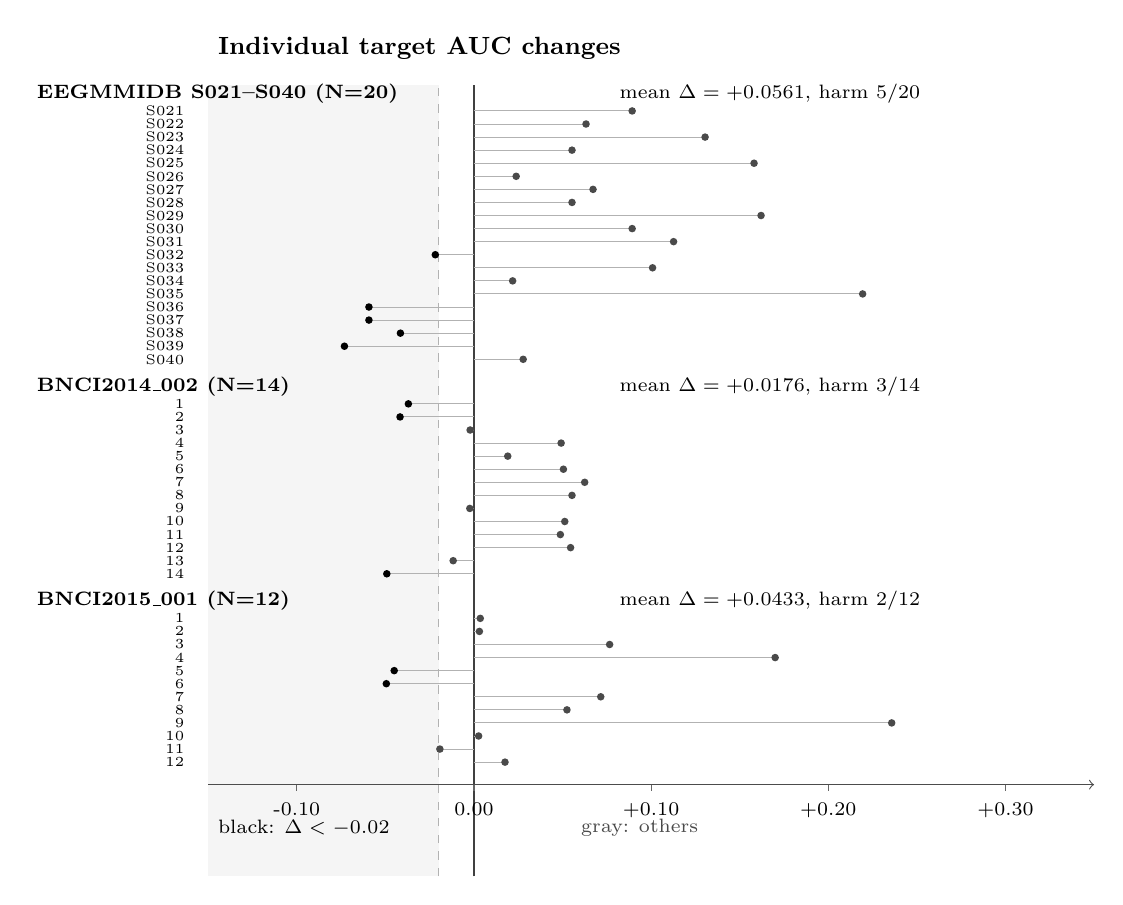
\begin{tikzpicture}[x=1cm,y=1cm]
\fill[gray!8] (2.300,1.68) rectangle (5.225,11.73);
\draw[dashed, gray!60] (5.225,1.68) -- (5.225,11.73);
\draw[black!75,line width=0.55pt] (5.675,1.68) -- (5.675,11.73);
\node[anchor=west,font=\small\bfseries] at (2.3,12.2) {Individual target AUC changes};
\node[anchor=west,font=\scriptsize\bfseries] at (0.0,11.620) {EEGMMIDB S021--S040 (N=20)};
\node[anchor=west,font=\scriptsize] at (7.4,11.620) {mean $\Delta=+0.0561$, harm 5/20};
\node[anchor=east,font=\tiny] at (2.12,11.400) {S021};
\draw[black!30,line width=0.35pt] (5.675,11.400) -- (7.684,11.400);
\fill[gray!58!black] (7.684,11.400) circle (0.048);
\node[anchor=east,font=\tiny] at (2.12,11.234) {S022};
\draw[black!30,line width=0.35pt] (5.675,11.234) -- (7.098,11.234);
\fill[gray!58!black] (7.098,11.234) circle (0.048);
\node[anchor=east,font=\tiny] at (2.12,11.068) {S023};
\draw[black!30,line width=0.35pt] (5.675,11.068) -- (8.610,11.068);
\fill[gray!58!black] (8.610,11.068) circle (0.048);
\node[anchor=east,font=\tiny] at (2.12,10.902) {S024};
\draw[black!30,line width=0.35pt] (5.675,10.902) -- (6.920,10.902);
\fill[gray!58!black] (6.920,10.902) circle (0.048);
\node[anchor=east,font=\tiny] at (2.12,10.736) {S025};
\draw[black!30,line width=0.35pt] (5.675,10.736) -- (9.232,10.736);
\fill[gray!58!black] (9.232,10.736) circle (0.048);
\node[anchor=east,font=\tiny] at (2.12,10.570) {S026};
\draw[black!30,line width=0.35pt] (5.675,10.570) -- (6.211,10.570);
\fill[gray!58!black] (6.211,10.570) circle (0.048);
\node[anchor=east,font=\tiny] at (2.12,10.404) {S027};
\draw[black!30,line width=0.35pt] (5.675,10.404) -- (7.187,10.404);
\fill[gray!58!black] (7.187,10.404) circle (0.048);
\node[anchor=east,font=\tiny] at (2.12,10.238) {S028};
\draw[black!30,line width=0.35pt] (5.675,10.238) -- (6.920,10.238);
\fill[gray!58!black] (6.920,10.238) circle (0.048);
\node[anchor=east,font=\tiny] at (2.12,10.072) {S029};
\draw[black!30,line width=0.35pt] (5.675,10.072) -- (9.321,10.072);
\fill[gray!58!black] (9.321,10.072) circle (0.048);
\node[anchor=east,font=\tiny] at (2.12,9.906) {S030};
\draw[black!30,line width=0.35pt] (5.675,9.906) -- (7.684,9.906);
\fill[gray!58!black] (7.684,9.906) circle (0.048);
\node[anchor=east,font=\tiny] at (2.12,9.740) {S031};
\draw[black!30,line width=0.35pt] (5.675,9.740) -- (8.210,9.740);
\fill[gray!58!black] (8.210,9.740) circle (0.048);
\node[anchor=east,font=\tiny] at (2.12,9.574) {S032};
\draw[black!30,line width=0.35pt] (5.675,9.574) -- (5.184,9.574);
\fill[black] (5.184,9.574) circle (0.048);
\node[anchor=east,font=\tiny] at (2.12,9.408) {S033};
\draw[black!30,line width=0.35pt] (5.675,9.408) -- (7.943,9.408);
\fill[gray!58!black] (7.943,9.408) circle (0.048);
\node[anchor=east,font=\tiny] at (2.12,9.242) {S034};
\draw[black!30,line width=0.35pt] (5.675,9.242) -- (6.166,9.242);
\fill[gray!58!black] (6.166,9.242) circle (0.048);
\node[anchor=east,font=\tiny] at (2.12,9.076) {S035};
\draw[black!30,line width=0.35pt] (5.675,9.076) -- (10.611,9.076);
\fill[gray!58!black] (10.611,9.076) circle (0.048);
\node[anchor=east,font=\tiny] at (2.12,8.910) {S036};
\draw[black!30,line width=0.35pt] (5.675,8.910) -- (4.341,8.910);
\fill[black] (4.341,8.910) circle (0.048);
\node[anchor=east,font=\tiny] at (2.12,8.744) {S037};
\draw[black!30,line width=0.35pt] (5.675,8.744) -- (4.341,8.744);
\fill[black] (4.341,8.744) circle (0.048);
\node[anchor=east,font=\tiny] at (2.12,8.578) {S038};
\draw[black!30,line width=0.35pt] (5.675,8.578) -- (4.741,8.578);
\fill[black] (4.741,8.578) circle (0.048);
\node[anchor=east,font=\tiny] at (2.12,8.412) {S039};
\draw[black!30,line width=0.35pt] (5.675,8.412) -- (4.030,8.412);
\fill[black] (4.030,8.412) circle (0.048);
\node[anchor=east,font=\tiny] at (2.12,8.246) {S040};
\draw[black!30,line width=0.35pt] (5.675,8.246) -- (6.300,8.246);
\fill[gray!58!black] (6.300,8.246) circle (0.048);
\node[anchor=west,font=\scriptsize\bfseries] at (0.0,7.900) {BNCI2014\_002 (N=14)};
\node[anchor=west,font=\scriptsize] at (7.4,7.900) {mean $\Delta=+0.0176$, harm 3/14};
\node[anchor=east,font=\tiny] at (2.12,7.680) {1};
\draw[black!30,line width=0.35pt] (5.675,7.680) -- (4.842,7.680);
\fill[black] (4.842,7.680) circle (0.048);
\node[anchor=east,font=\tiny] at (2.12,7.514) {2};
\draw[black!30,line width=0.35pt] (5.675,7.514) -- (4.736,7.514);
\fill[black] (4.736,7.514) circle (0.048);
\node[anchor=east,font=\tiny] at (2.12,7.348) {3};
\draw[black!30,line width=0.35pt] (5.675,7.348) -- (5.626,7.348);
\fill[gray!58!black] (5.626,7.348) circle (0.048);
\node[anchor=east,font=\tiny] at (2.12,7.182) {4};
\draw[black!30,line width=0.35pt] (5.675,7.182) -- (6.782,7.182);
\fill[gray!58!black] (6.782,7.182) circle (0.048);
\node[anchor=east,font=\tiny] at (2.12,7.016) {5};
\draw[black!30,line width=0.35pt] (5.675,7.016) -- (6.104,7.016);
\fill[gray!58!black] (6.104,7.016) circle (0.048);
\node[anchor=east,font=\tiny] at (2.12,6.850) {6};
\draw[black!30,line width=0.35pt] (5.675,6.850) -- (6.811,6.850);
\fill[gray!58!black] (6.811,6.850) circle (0.048);
\node[anchor=east,font=\tiny] at (2.12,6.684) {7};
\draw[black!30,line width=0.35pt] (5.675,6.684) -- (7.081,6.684);
\fill[gray!58!black] (7.081,6.684) circle (0.048);
\node[anchor=east,font=\tiny] at (2.12,6.518) {8};
\draw[black!30,line width=0.35pt] (5.675,6.518) -- (6.920,6.518);
\fill[gray!58!black] (6.920,6.518) circle (0.048);
\node[anchor=east,font=\tiny] at (2.12,6.352) {9};
\draw[black!30,line width=0.35pt] (5.675,6.352) -- (5.622,6.352);
\fill[gray!58!black] (5.622,6.352) circle (0.048);
\node[anchor=east,font=\tiny] at (2.12,6.186) {10};
\draw[black!30,line width=0.35pt] (5.675,6.186) -- (6.828,6.186);
\fill[gray!58!black] (6.828,6.186) circle (0.048);
\node[anchor=east,font=\tiny] at (2.12,6.020) {11};
\draw[black!30,line width=0.35pt] (5.675,6.020) -- (6.772,6.020);
\fill[gray!58!black] (6.772,6.020) circle (0.048);
\node[anchor=east,font=\tiny] at (2.12,5.854) {12};
\draw[black!30,line width=0.35pt] (5.675,5.854) -- (6.902,5.854);
\fill[gray!58!black] (6.902,5.854) circle (0.048);
\node[anchor=east,font=\tiny] at (2.12,5.688) {13};
\draw[black!30,line width=0.35pt] (5.675,5.688) -- (5.411,5.688);
\fill[gray!58!black] (5.411,5.688) circle (0.048);
\node[anchor=east,font=\tiny] at (2.12,5.522) {14};
\draw[black!30,line width=0.35pt] (5.675,5.522) -- (4.568,5.522);
\fill[black] (4.568,5.522) circle (0.048);
\node[anchor=west,font=\scriptsize\bfseries] at (0.0,5.176) {BNCI2015\_001 (N=12)};
\node[anchor=west,font=\scriptsize] at (7.4,5.176) {mean $\Delta=+0.0433$, harm 2/12};
\node[anchor=east,font=\tiny] at (2.12,4.956) {1};
\draw[black!30,line width=0.35pt] (5.675,4.956) -- (5.755,4.956);
\fill[gray!58!black] (5.755,4.956) circle (0.048);
\node[anchor=east,font=\tiny] at (2.12,4.790) {2};
\draw[black!30,line width=0.35pt] (5.675,4.790) -- (5.744,4.790);
\fill[gray!58!black] (5.744,4.790) circle (0.048);
\node[anchor=east,font=\tiny] at (2.12,4.624) {3};
\draw[black!30,line width=0.35pt] (5.675,4.624) -- (7.398,4.624);
\fill[gray!58!black] (7.398,4.624) circle (0.048);
\node[anchor=east,font=\tiny] at (2.12,4.458) {4};
\draw[black!30,line width=0.35pt] (5.675,4.458) -- (9.500,4.458);
\fill[gray!58!black] (9.500,4.458) circle (0.048);
\node[anchor=east,font=\tiny] at (2.12,4.292) {5};
\draw[black!30,line width=0.35pt] (5.675,4.292) -- (4.662,4.292);
\fill[black] (4.662,4.292) circle (0.048);
\node[anchor=east,font=\tiny] at (2.12,4.126) {6};
\draw[black!30,line width=0.35pt] (5.675,4.126) -- (4.562,4.126);
\fill[black] (4.562,4.126) circle (0.048);
\node[anchor=east,font=\tiny] at (2.12,3.960) {7};
\draw[black!30,line width=0.35pt] (5.675,3.960) -- (7.285,3.960);
\fill[gray!58!black] (7.285,3.960) circle (0.048);
\node[anchor=east,font=\tiny] at (2.12,3.794) {8};
\draw[black!30,line width=0.35pt] (5.675,3.794) -- (6.856,3.794);
\fill[gray!58!black] (6.856,3.794) circle (0.048);
\node[anchor=east,font=\tiny] at (2.12,3.628) {9};
\draw[black!30,line width=0.35pt] (5.675,3.628) -- (10.980,3.628);
\fill[gray!58!black] (10.980,3.628) circle (0.048);
\node[anchor=east,font=\tiny] at (2.12,3.462) {10};
\draw[black!30,line width=0.35pt] (5.675,3.462) -- (5.734,3.462);
\fill[gray!58!black] (5.734,3.462) circle (0.048);
\node[anchor=east,font=\tiny] at (2.12,3.296) {11};
\draw[black!30,line width=0.35pt] (5.675,3.296) -- (5.242,3.296);
\fill[gray!58!black] (5.242,3.296) circle (0.048);
\node[anchor=east,font=\tiny] at (2.12,3.130) {12};
\draw[black!30,line width=0.35pt] (5.675,3.130) -- (6.069,3.130);
\fill[gray!58!black] (6.069,3.130) circle (0.048);
\draw[->,black!70] (2.300,2.844) -- (13.550,2.844);
\draw[black!60] (3.425,2.844) -- (3.425,2.764);
\node[anchor=north,font=\scriptsize] at (3.425,2.734) {-0.10};
\draw[black!60] (5.675,2.844) -- (5.675,2.764);
\node[anchor=north,font=\scriptsize] at (5.675,2.734) {0.00};
\draw[black!60] (7.925,2.844) -- (7.925,2.764);
\node[anchor=north,font=\scriptsize] at (7.925,2.734) {+0.10};
\draw[black!60] (10.175,2.844) -- (10.175,2.764);
\node[anchor=north,font=\scriptsize] at (10.175,2.734) {+0.20};
\draw[black!60] (12.425,2.844) -- (12.425,2.764);
\node[anchor=north,font=\scriptsize] at (12.425,2.734) {+0.30};
\node[anchor=west,font=\scriptsize,black] at (2.300,2.294) {black: $\Delta<-0.02$};
\node[anchor=west,font=\scriptsize,gray!58!black] at (6.912,2.294) {gray: others};
\end{tikzpicture}
\caption{Paired participant-level target AUC differences between the frozen source participant-macro selector and the historical class-centred CovScore selector in three EEG cohorts. Five of 20, three of 14 and two of 12 participants, respectively, lost more than 0.02 AUC. The vertical reference line is zero, and the tinted region denotes the material-harm threshold. All three cohorts had been previously examined at project level; a within-run source lock does not turn the participant effects into externally preregistered confirmations. Historical Holm-adjusted results remain retrospective evidence. Points are descriptive and must not be treated as independent trials or a new confirmatory family.}
\label{fig:participant-harm-v10}
\end{figure*}


\subsection{Retrospective real-EEG check of the properly predictive comparator}
\label{sec:v18-fair-predictive}
The original class-centred comparator does not account for
between-source-person class-mean shifts
(Section~\ref{sec:v17-mean-shift-decomposition}, Eq.~\eqref{eq:v17-exact-nll-shift}).
We therefore executed a \emph{new secondary, post-outcome} comparison
of the correctly defined $C_{\mathrm{pred}}$ selector on public
Shin2017A EEG using the original, independent previously executed
preprocessing and classifier implementation. This additional
analysis is neither a new dataset nor a renewal of the earlier
confirmatory study. The Shin2017A outcomes had been seen before
the new score was specified.

For each of 29 outer held participants, the entire source-only
tangent reference and within-class state were reconstructed using
the other 28 participants. The source-participant-grouped inner
validation used only source-person trial labels; for each held
\emph{source} validation fold, the class means appearing in
Eq.~\eqref{eq:v16-conditional-prediction} were fitted exclusively
on the corresponding inner \emph{training} source groups.
The candidate set was that fold's originally source-feasible
27-point shrinkage grid, and the per-person proper-predictive
Gaussian log scores were averaged with equal source-person
weight. All 29 selected shrinkage strengths were serialised to
a machine-readable file and locked with SHA-256
\texttt{fac20e7f1ec1e43f3fa01af8ce88e44869e80f624d9a10b6123a57a6687f9b5c}
before re-opening the immutable original ZIP and reading the
outer target AUC outcomes. The original class-centred comparator
and source-macro policy were unchanged; the original Shin
score archive retained its previously verified SHA-256.



We also compared the two source-validation score
paths themselves, at the \emph{same} $\lambda=0.2$,
using the immutable original and new source-grouped
receipts. The genuine predictive Gaussian log score
exceeded the validation-class-centred covariance score
in 29/29 outer training pools. The mean difference
was $+0.86995$ per feature, ranging from $+0.83371$
to $+0.94214$. This is the nonnegative class-mean
shift penalty of Eq.~\eqref{eq:v17-exact-nll-shift}
measured on \emph{real EEG source validation data}.
These 29 source pools overlap heavily; neither their
positive signs nor the numerical penalty imply
a new independent dataset replication or a causal
guarantee of higher held-person AUC.

The newly implemented proper-predictive objective selected
\(\lambda=0.2\) in \emph{all 29} outer folds. It differs from the
original class-centred covariance choice in 29/29 folds, yet its
person-macro target AUC of \(0.786207\) was almost identical
to the source-macro policy's \(0.785900\). Proper predictive
scoring exceeded the original class-centred covariance
selection by \(0.022529\) person-macro AUC. In this
single previously exposed EEG dataset, the large comparison
against the class-centred score therefore does
\emph{not} translate into a discrimination-selector advantage
against genuine predictive likelihood.

The agreement between the two better-performing methods
should not be misrepresented as a general statistical
equivalence or proven non-inferiority. The new result
contains no new hypothesis test or adjusted $p$-value,
and equal source-population folds remain strongly dependent.
All 29 proper-predictive choices being 0.2 demonstrates
\emph{selection stability on highly overlapping training pools},
not successful participant-specific adaptation.
This new comparison narrows the paper's conclusion to
the \emph{measurement target itself}: a held-source
class-centred covariance log score can omit the
class-mean-shift penalty, changing the selected
regularisation regime and biasing the interpretation
of EEG decoding method comparisons.


\subsection{Second real EEG source-mean predictive comparison}
\label{sec:v18-bnci-proper}
We repeated the corrected source-mean Gaussian predictive
criterion on the \emph{original, separately frozen}
BNCI2014\_002 frontier experiment. Its public EEG pipeline
contained 14 held persons, 2240 trials and the original
source-only tangent-LDA scoring family. The new analysis
was specified \emph{after} this dataset's outcomes were
available; thus the original experiment's true-pre-data
status does not carry over to the new comparator.
The corresponding original artifact and new source-choice
files were independently read, with 14 paired AUC values
verified against the original immutable target AUC paths.

\begin{table}[tb]
\centering
\small
\caption{Matched real EEG descriptive comparisons after
correcting the covariance validation estimand. Entries
for the properly predictive criterion are \emph{post-outcome}
secondary analyses. The two rows correspond to different
public datasets, not two independent pre-data confirmations
of the new criterion. Mean source log-score penalty is
\(C_{\rm pred}-C_{\rm cent}\) at the newly chosen shrinkage
value, normalised per feature; positive values are an
exact class-mean-shift consequence.}
\label{tab:v18-two-real-cohorts}
\begin{tabular}{lcc}
\toprule
Metric & Shin2017A & BNCI2014\_002\\
\midrule
Held persons & 29 & 14\\
Source-macro selected AUC & 0.785900 & 0.778705\\
Proper predictive selected AUC & 0.786207 & 0.771886\\
Historical class-centred AUC & 0.763678 & 0.761116\\
Macro minus proper AUC & $-0.000307$ & $+0.006819$\\
Proper minus historical AUC & $+0.022529$ & $+0.010770$\\
Mean source class-mean-shift penalty & $+0.86995$ & $+0.91218$\\
Positive source penalties / folds & 29/29 & 14/14\\
\bottomrule
\end{tabular}
\end{table}

On BNCI2014\_002, the corrected proper-predictive
criterion selected \(\lambda=0.3\) in five folds,
\(0.4\) in eight, and \(0.5\) in one, contrasting
with the uniform \(0.2\) on Shin2017A.
Its person-macro AUC was \(0.771886\), compared
with \(0.778705\) under source-macro selection.
The difference of \(+0.006819\) AUC in favour
of source-macro selection is \emph{descriptive}.
An exploratory bootstrap over the 14 held persons,
conditional on their overlapping source fits,
gave the interval \([-0.00595,0.02027]\) AUC,
which includes zero. It cannot be interpreted
as a predeclared test, an equivalence result or
a population-level confidence interval.

At the same chosen \(\lambda\) within each
outer fold, the proper source log score
was higher than the class-centred score in
14/14 folds. The mean nonnegative difference
was \(+0.91218\) per feature, with foldwise
range \(+0.86056\) to \(+1.00008\).
This observation supports the algebraic
source-mean-shift decomposition in a second
public EEG dataset; it does \emph{not}
establish that the penalty predicts the
direction of target AUC gains.

The original BNCI2014\_002 frontier archive
used in this secondary comparison has its
own stored source-selection settings and
reported AUCs. It must not be silently
substituted for the separate originally frozen
two-BNCI testing-family statistics reported
above (for example, their originally
adjusted nonsignificant tests). Both
pre-existing score families are preserved
under their exact artifact identities,
and the corrected baseline is not added
retroactively to either family.




\subsection{A low-dimensional, risk-aware EEG stress test}
\label{sec:v21-lowrank-risk}
To challenge the possibility that the
estimand effect requires very high dimensionality,
we independently tested BNCI2014\_004,
BCI Competition IV Dataset 2b,
containing three bipolar EEG channels
and six covariance-tangent coordinates
\cite{tangermann2012bciiv,jayaram2018moabb}.
The 2026-10-12 repository-frozen first-run
protocol held each of nine people out,
using all available sessions. MOABB 1.7.2
returned 6,520 balanced trials (680--760
per person). These are measured per-person
counts, not the nominal catalogue total.

As a source-subject downside-risk
stress test, we added the following
fixed selector, alongside the original
macro-AUC, genuine source-mean Gaussian
predictive and historical validation
class-centred covariance scores:
\[
\widehat\lambda_{\mathrm{CVaR}}=
\arg\max_{\lambda\in\Lambda_{\rm src}}
\frac{A^{\rm src}_{(1)}(\lambda)+
A^{\rm src}_{(2)}(\lambda)}2 .
\]
Here $A^{\rm src}_{(j)}$ is the
$j$-th smallest held-source-person AUC
among eight SOURCE people in the fixed
five grouped folds. This is a
conventional worst-quarter CVaR
risk functional, \emph{not} an
independently novel learning operator.
Source-only choice vectors were SHA-256
locked before outer target AUC computation,
and the policy/grid were fixed before
this run. No target data entered model
or regularisation selection.

\begin{table}[tb]
\centering\small
\caption{New BNCI2014\_004 source-only
evaluation (9 people; 6,520 held-person
trials; 3 EEG channels, 6 tangent features).
All gains are descriptive, not independently
preregistered confirmation. CVaR stress
testing is a source-domain baseline.}
\label{tab:v21-lowdim-cvar}
\begin{tabular}{lr}
\toprule
Selection criterion & Mean AUC\\
\midrule
Held-source-person macro-AUC & 0.778002\\
Proper source-mean predictive Gaussian score & 0.776581\\
Worst-quarter source AUC (CVaR) & 0.777141\\
Historical source class-centred covariance & 0.770549\\
Ledoit--Wolf & 0.770628\\
OAS & 0.770640\\
\midrule
CVaR minus macro & $-0.000861$\\
CVaR minus macro, conditional bootstrap 95\% &
$[-0.00358,0.00067]$\\
CVaR selected a different $\lambda$ & 8/9 folds\\
$>0.02$ AUC harms relative to macro & 0/9\\
\bottomrule
\end{tabular}
\end{table}

The historical covariance criterion
selected $\lambda=0$ in all nine
source pools. The correctly predictive
Gaussian criterion selected 0.10--0.30
and source-macro discrimination
selected 0.50--0.80. The source CVaR
criterion changed the lambda choice
in 8/9 folds but \emph{did not
improve} mean held-person AUC,
nor the count of subject harms above
0.02 AUC. The class-mean-shift source
log-score penalty, evaluated at
properly selected shrinkage, was
nonnegative as required by algebra,
with empirical mean 0.92622 per feature.

These observations extend the
\emph{decision-instability mechanism}
to very low dimensional EEG geometry,
but reject a simplistic assumption
that source downside-risk optimization
must improve unseen-person AUC.
All nine source pools overlap and
there is one acquisition dataset,
not nine independent sites. The
protocol was committed before the
run, but was not independently
preregistered.

\subsection{Independent-acquisition Weibo2014 source-locked test: no gain from finer optimisation}
\label{sec:v24-weibo}
The repository-fixed V24 first-run protocol specified Weibo2014
\cite{yi2014simplecompound,jayaram2018moabb} before any newly acquired
target outcomes were evaluated. It used all ten participants, the
fixed C3/Cz/C4 three-channel sensorimotor subset, left- versus
right-hand motor imagery, 8--30 Hz processing and a 160 Hz resample.
All 1,580 actually loaded trials were retained. This is a
different acquisition from the original cohorts, but deliberately
restricted to six covariance-tangent features and one binary task.
It is not an independent preregistered clinical trial.

All ten outer-held-person source-only parameter vectors were saved
and SHA-256 hashed before \emph{any} target scores were calculated.
The original 27-point held-source macro-AUC shrinkage choice,
a same-range, baseline-anchored continuous source optimiser,
source-trained-mean predictive Gaussian NLL, the historical
validation-class-centred covariance score, Ledoit--Wolf, OAS
and fixed $\lambda=0.50$ were evaluated on identical held-person
trials using the original tangent-LDA pipeline.

\begin{table}[tb]
\centering\small
\caption{V24 new Weibo2014 acquisition: mean held-person ROC-AUC,
$N=10$ people and 1,580 original MI trials. Models have identical
three-channel geometry and target information access (Z0).
These are descriptive first-run results, not independently
preregistered confirmation.}
\label{tab:v24-weibo}
\begin{tabular}{lr}
\toprule
Source-only selection policy & Held-person macro AUC\\
\midrule
Original 27-point source macro-AUC & 0.731405\\
V24 anchored continuous source AUC & 0.731405\\
Fixed $\lambda=0.50$ & 0.730149\\
Correct source-trained-mean Gaussian predictive NLL & 0.729358\\
Ledoit--Wolf & 0.725509\\
OAS & 0.725509\\
Historical validation-class-centred covariance & 0.725489\\
\midrule
V24 minus original grid & $0.000000$\\
V24 minus proper predictive NLL & $+0.002047$\\
\bottomrule
\end{tabular}
\end{table}

The conditional source-optimisation residual was at most
0.02 AUC on \emph{all ten} outer source pools, yet the
continuous optimiser selected the \emph{identical}
$\lambda$ as the 27-point source-macro baseline in
10/10 cases. The held-person AUC advantage over that
baseline was exactly zero in every person. Neither
method harmed a held individual by more than 0.02 AUC
relative to the other because their decisions were
identical. Against the correctly predictive Gaussian
selection, V24 had mean difference $+0.002047$; a
descriptive participant bootstrap interval was
$[-0.000234,0.004219]$, including zero. The corresponding
difference versus the historical class-centred score
was $+0.005916$; no individual difference in that
comparison exceeded 0.02 AUC in absolute magnitude.
The bootstrap intervals are conditional descriptive
statistics from ten overlapping-source LOSO fits;
they are \emph{not} a confirmatory population test.

This negative optimisation result is consequential:
more precise optimisation of a correctly defined
\emph{source} ranking criterion cannot be assumed
to yield a meaningfully better unknown-person
decoder. The result is consistent with the
distinction in Eq.~\eqref{eq:v24-transfer-gap},
but a small difference between policies alone
does not identify a causal mechanism of transfer.
We do not promote continuous optimisation to a
superior transfer algorithm.

An independent verifier downloaded the original
first-run Actions artifact, rechecked the ten
source-person selection records, recomputed all
held-person AUC macro means and the paired descriptive
statistics, and verified the pre-target selection
hash. The source-choice SHA-256 is
\texttt{a2fb5b334218a00b\ldots} (full digest in the online evidence ledger).
The original first-run Actions identifier is
\texttt{38279322314}; the independent verification
identifier is \texttt{38280133125}. The outcome
receipt was not used to revise the precommitted
selector or protocol. The acquisition/source
validity of its data is constrained by the
public dataset loader, not an independent
recollection of EEG.

% Frozen V31 first-run Cho2017 after independent immutable artifact audit.
% An observed SMALL, NONSIGNIFICANT positive contrast; no SOTA claim.
\subsection{Independent-acquisition stress test of a source-contrast envelope}
\label{sec:v31-cho}
The source-contrast envelope (Section~\ref{sec:v31-brief-method})
was precommitted before reading 20 target-person recordings from
the public Cho2017 acquisition. Exactly 12 other source persons
were used for every source-only choice; the outer targets
13--32 contributed 4,000 motor-imagery trials and were accessed
only after SHA-256 locking of the source manifest.
All methods used the fixed C3/Cz/C4 montage, 8--30 Hz band
and identical pooled-LDA spectral score family.
The old source macro-AUC 27-point grid selected $\lambda=0.5$,
the new $\rho=1$ source-envelope method selected $\lambda=1$,
the radius-zero geometric ablation selected $\lambda=0.3$,
and the properly predictive Gaussian source NLL selected $\lambda=0.1$.
The source-only pairwise dominance test did not certify
the new choice against the original macro-grid one.

\begin{table}[ht]
\centering
\small
\caption{Cho2017 externally held-person macro ROC-AUC.
The original source-macro criterion is the sole predefined
reference for the new SCE method. Other rows are descriptive controls;
all decisions were fixed before opening target outcomes.}
\label{tab:v31-cho}
\begin{tabular}{lr}
\toprule
Source-only regularisation choice & Macro AUC\\
\midrule
Source contrast envelope (SCE, $\rho=1$) & 0.618230\\
Original source-macro full grid & 0.614835\\
SCE radius-zero ablation ($\rho=0$) & 0.610300\\
Proper source-mean Gaussian NLL & 0.601830\\
OAS & 0.593580\\
Ledoit--Wolf & 0.593535\\
Historical validation-class-centred likelihood & 0.593355\\
\bottomrule
\end{tabular}
\end{table}
The paired difference, SCE minus the original source-macro
selector, was $+0.003395$ AUC. Fourteen persons improved and
six declined; none improved or declined by more than 0.02 AUC.
The descriptive 20,000-draw participant bootstrap 95\% interval
contained zero:
\[
[-0.000295,\ 0.006975].
\]
The two-sided all-$2^{20}$-sign enumeration gave
$p=0.0930843$ under the usual sign-flip reference assumptions;
thus this predeclared positive-method promotion gate FAILED.
The subject-level inference depends on the paired-sign symmetry
assumption, not trial pseudo-replication, and no external
preregistration or clinical utility is claimed.

This result is especially important because the new method
chose the upper shrinkage endpoint $\lambda=1$.
Its slight mean advantage in one acquisition does not establish
that the across-source contrast ellipsoid is a calibrated
future-person uncertainty set, that the source-only certificate
correctly predicts individual benefit, or that the new
selection policy is robust across recording conditions.
Both the all-person first-run result and the non-positive
inferential conclusion are kept; the V31 method is not promoted
to the primary manuscript contribution.

% V31B reserved block was SEQUENTIAL/POST-FIRST-BLOCK protocol,
% NOT a second acquisition or independent preregistration.
\subsection{The identical frozen SCE choice reverses on reserved participants}
\label{sec:v31b-cho40}
After seeing the initial Cho2017 participant outcomes, we
committed a \emph{sequential, exploratory} reserved-person protocol
for the 20 remaining identifiers 33--52. The original
source IDs 1--12, source preprocessing, and algorithm code
were reused without any tuning or changed feature
configuration. Before reading any reserved target EEG,
the source-choice manifest was regenerated and required
to be byte-identical to the first-run manifest
(SHA-256 prefix \texttt{677f848de0e3}).
All selected parameters matched exactly; in particular
the SCE $\rho=1$ choice stayed $\lambda=1.0$ and the
original source-macro grid stayed $\lambda=0.5$.

\begin{table}[ht]
\centering
\small
\caption{Cho2017 held-person ROC-AUC under the same source-only
classifier fit and choices. The second block is a
\emph{sequential follow-up within one acquisition},
not a newly independent dataset. The primary original
first-run outcome did not attain its planned threshold.}
\label{tab:v31b-cho40}
\begin{tabular}{lccc}
\toprule
Method & First 20 & Reserved 20 & All 40\\
\midrule
Source envelope $\rho=1$ & 0.618230 & 0.615761 & 0.616996\\
Original source-macro grid & 0.614835 & 0.619261 & 0.617048\\
Envelope $\rho=0$ & 0.610300 & 0.618997 & 0.614648\\
Proper Gaussian source NLL & 0.601830 & 0.615487 & 0.608658\\
Analytic Ledoit--Wolf & 0.593535 & 0.609938 & 0.601736\\
Analytic OAS & 0.593580 & 0.609954 & 0.601767\\
Historical class-centred NLL & 0.593355 & 0.609807 & 0.601581\\
\midrule
SCE minus original grid & +0.003395 & -0.003500 & -0.000053\\
\bottomrule
\end{tabular}
\end{table}

The 20 reserved persons contributed another 4,040 held EEG
trials. SCE lost $0.003500$ participant-macro AUC relative
to the unchanged baseline and harmed one participant by
more than $0.02$ AUC. The within-block descriptive
two-sided paired sign-flip reference was $p=0.166742$.
The original first-block gain was only $+0.003395$.
Together all 40 held persons (8,040 trials) show
a near-zero macro contrast, $-0.00005264$ AUC,
with a descriptive participant-bootstrap 95\% interval
$[-0.003218,0.002973]$ and an exploratory
Monte Carlo sign-flip reference of approximately $0.974$.
The latter is \emph{not} a predeclared independent
confirmatory $p$ value because the follow-up itself was
specified after the first block was seen.
The two target blocks share the same source model and
acquisition; they cannot be counted as two independently
collected experiments.

There is a more basic algorithmic falsification: at the
selected $\lambda_{\mathrm{SCE}}=1$, the pooled LDA path has
$A_1=\nu I$ and $w_1=d_{\mathrm{pooled}}/\nu$.
Consequently its target scores and all ROC-AUC ranks
are exactly those of an \emph{untuned fixed
$\lambda=1$} full-shrinkage LDA, up to a positive
scale. Thus the Cho2017 results do not establish
any added classifier value from the SCE ellipsoid
over the trivial fixed endpoint. A source-only
conditional guarantee of superiority over the
original grid was also not obtained.

The source-group ellipsoid and a pre-outcome locked
choice therefore did not suffice to predict a stable
advantage in this public acquisition. Even though the
first 20-person result was positive, it did not survive
an identical-code no-retuning follow-up. This falsifies
promotion of SCE as a reliably better regularisation
selector based on the current evidence. The exact
ellipsoid minimum and worst-case witness remain
\emph{conditional theoretical tools}, not empirical
cross-subject performance certificates.


\subsection{The key prospective spectral-representation prediction fails}
On the separate untouched S041--S060 block, four prespecified
configurations compared WIDE231, FB8-1848, source-PCA-matched
FB8-231 and nuisance-augmented WIDE-1848. The primary
difference-in-differences for FB8-vs-WIDE under discrimination versus
Ledoit--Wolf regularisation was \(-0.07781\) AUC
(95\% [-0.12415,-0.03451], Holm \(p=0.01328\)).
The selection objective materially affected the representation
conclusion, but in the \emph{opposite} direction to the historical
claim that discrimination-oriented regularisation would reveal a
universal filter-bank advantage. Dimensionality-matched and nuisance
controls also contradicted a monotonic feature-dimension explanation.

\section{Discussion}
The central finding is not that discrimination-optimised covariance
shrinkage is universally preferable, but that \emph{an apparently
reasonable validation criterion can silently change the scientific
estimand}. The previously called Cov-NLL scored each held-source
participant after subtracting that participant's own validation-class
means. It therefore omitted an exact, nonnegative source-trained-mean
shift penalty and must not be compared to discriminative selection
as if it were proper predictive likelihood. The corrected source-trained
Gaussian score changes the magnitude and interpretation of the earlier
advantage. Selecting shrinkage using held-source discrimination is
classical; our contribution concerns the reproducibility and
interpretation of that objective comparison, not priority for
discriminative tuning \cite{friedman1989,tomioka2010regularized}.

The prospectively fixed EEGMMIDB comparison is real, but it also
contains harmed participants; the two original independently frozen
BNCI families do not individually establish adjusted superiority.
Shin2017A's proper predictive comparison is retrospective.
The subsequent three-channel CVaR experiment demonstrated
that changing the source-selected regularisation does not
necessarily change target discrimination, and the prospective
spectral-representation intervention refuted the initially
expected universal filter-bank advantage. These negative
results are central to the paper, not unsuccessful parameter
searches to be discarded.

The V22 and V23 mechanisms distinguish source parameter changes,
score-pair order changes and source-validation AUC effects.
The V24 continuous branch-and-bound repair provides a useful
conditional finite-\emph{source} optimisation gap. Yet the new
Weibo2014 experiment is more informative for its \emph{failure
to improve transfer}: the same shrinkage was selected
in every outer source pool by the new continuous method
and the original 27-point grid, producing identical
held-person predictions by that pipeline. The average
$+0.00205$ AUC contrast to proper predictive likelihood
has a descriptive participant interval containing zero.
Under the deterministic decomposition of
Eq.~\eqref{eq:v24-transfer-gap}, closing the source
optimisation term cannot bound the unobserved
source--target discrepancy; no source-only rank
certificate is an unseen-person safety guarantee.

A second newly evaluated acquisition, Cho2017, adds a
source-locked robustness challenge beyond merely searching
the finite shrinkage grid more exactly
(Section~\ref{sec:v31-cho}). Although the predeclared SCE
source-contrast operator obtained a $+0.003395$ AUC
difference versus the original source-macro choice,
its sign-flip reference result ($p=0.0931$) and
participant-bootstrap interval crossing zero do not
establish a genuine positive transfer benefit.
The source-only dominance check was negative, and the
chosen $\lambda=1$ indicates potential boundary saturation.
We therefore use SCE as a falsification probe rather than
an advertised superior EEG decoder.

The independent Weibo acquisition extends the practical
stress test to another recording site, but the fixed
three-channel, single binary MI task is deliberately
limited. Its ten overlapping-source leave-one-person-out
models do not provide ten independent study replications,
and repository protocol-first chronology is weaker than
independent preregistration. The work does not establish
SOTA deep EEG performance, calibration time saved,
clinical safety, or deployment-ready trigger policies.
The most robust methodological recommendation is to
specify validation estimands, target-information budgets,
pre-outcome selection boundaries, negative controls,
and participant-level adverse effects before making
claims about EEG regularisation.

\section{Conclusion}
An historical validation-class-centred EEG covariance score
was not a proper predictive Gaussian likelihood, and
the distinction changes how earlier discrimination-based
regularisation gains should be interpreted. Exact
pairwise ranking and spectral path analyses clarify why
source selection decisions can differ without producing
important target AUC improvements. The independently
audited ten-person Weibo2014 protocol-first test
found that source-optimality gaps were numerically
small but continuous selection and the original
27-point source grid chose identical parameters and
achieved the same held-person macro AUC.
A further source-locked Cho2017 study of 40 target persons
gave opposite signed effects in two sequential 20-person
blocks, with effectively zero combined improvement under
identical source-only parameter choices. This strengthens
the conclusion that more elaborate source-only regularisation
does not reliably improve unknown-person transfer.
This supports \emph{measurement correctness and
selection validity} as the manuscript's contribution,
not superiority of a new EEG decoder. Broader
multi-acquisition, fully independent pre-data
replication is required before claiming a universally
safe or better shrinkage rule.

\section*{Statements and Declarations}
\textbf{Data availability:} The EEG cohorts are publicly distributed.
Original participant score receipts, repository commit hashes and code
availability must be confirmed in the final submission package.

\textbf{Author contribution, funding, competing interests, ethics and
AI-assisted writing:} To be completed and confirmed by all authors before
publisher upload. No declaration is made on an author's behalf.

\bibliographystyle{unsrt}
\bibliography{references_v10}
\end{document}
